% This file was created with tikzplotlib v0.10.1.
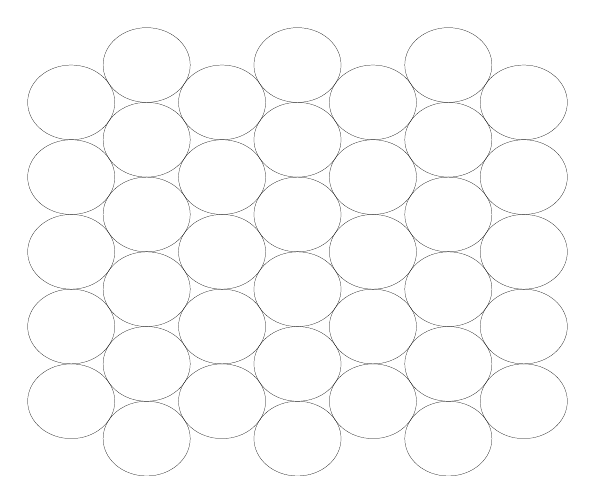
\begin{tikzpicture}

\definecolor{darkgray176}{RGB}{176,176,176}

\begin{axis}[
hide x axis,
hide y axis,
tick align=outside,
tick pos=left,
x grid style={darkgray176},
xmin=-0.929422863405995, xmax=0.929422863405995,
xtick style={color=black},
y grid style={darkgray176},
ymin=-0.9, ymax=0.9,
ytick style={color=black}
]
\draw[draw=black,line width=0.08pt] (axis cs:0,0.15) circle (0.15);
\draw[draw=black,line width=0.08pt] (axis cs:0,-0.15) circle (0.15);
\draw[draw=black,line width=0.08pt] (axis cs:-0.259807621135332,0) circle (0.15);
\draw[draw=black,line width=0.08pt] (axis cs:0.259807621135332,0) circle (0.15);
\draw[draw=black,line width=0.08pt] (axis cs:-0.259807621135332,0.3) circle (0.15);
\draw[draw=black,line width=0.08pt] (axis cs:-0.259807621135332,-0.3) circle (0.15);
\draw[draw=black,line width=0.08pt] (axis cs:0.259807621135332,0.3) circle (0.15);
\draw[draw=black,line width=0.08pt] (axis cs:0.259807621135332,-0.3) circle (0.15);
\draw[draw=black,line width=0.08pt] (axis cs:0,0.45) circle (0.15);
\draw[draw=black,line width=0.08pt] (axis cs:-0.519615242270663,0.15) circle (0.15);
\draw[draw=black,line width=0.08pt] (axis cs:0,-0.45) circle (0.15);
\draw[draw=black,line width=0.08pt] (axis cs:-0.519615242270663,-0.15) circle (0.15);
\draw[draw=black,line width=0.08pt] (axis cs:0.519615242270663,0.15) circle (0.15);
\draw[draw=black,line width=0.08pt] (axis cs:0.519615242270663,-0.15) circle (0.15);
\draw[draw=black,line width=0.08pt] (axis cs:-0.259807621135332,0.6) circle (0.15);
\draw[draw=black,line width=0.08pt] (axis cs:0.259807621135332,0.6) circle (0.15);
\draw[draw=black,line width=0.08pt] (axis cs:-0.519615242270663,0.45) circle (0.15);
\draw[draw=black,line width=0.08pt] (axis cs:-0.259807621135332,-0.6) circle (0.15);
\draw[draw=black,line width=0.08pt] (axis cs:0.259807621135332,-0.6) circle (0.15);
\draw[draw=black,line width=0.08pt] (axis cs:-0.519615242270663,-0.45) circle (0.15);
\draw[draw=black,line width=0.08pt] (axis cs:-0.779422863405995,0) circle (0.15);
\draw[draw=black,line width=0.08pt] (axis cs:0.519615242270663,0.45) circle (0.15);
\draw[draw=black,line width=0.08pt] (axis cs:0.519615242270663,-0.45) circle (0.15);
\draw[draw=black,line width=0.08pt] (axis cs:0.779422863405995,0) circle (0.15);
\draw[draw=black,line width=0.08pt] (axis cs:1.11022302462516e-16,0.75) circle (0.15);
\draw[draw=black,line width=0.08pt] (axis cs:-0.779422863405995,0.3) circle (0.15);
\draw[draw=black,line width=0.08pt] (axis cs:-0.519615242270663,0.75) circle (0.15);
\draw[draw=black,line width=0.08pt] (axis cs:1.11022302462516e-16,-0.75) circle (0.15);
\draw[draw=black,line width=0.08pt] (axis cs:-0.779422863405995,-0.3) circle (0.15);
\draw[draw=black,line width=0.08pt] (axis cs:-0.519615242270663,-0.75) circle (0.15);
\draw[draw=black,line width=0.08pt] (axis cs:0.779422863405995,0.3) circle (0.15);
\draw[draw=black,line width=0.08pt] (axis cs:0.519615242270663,0.75) circle (0.15);
\draw[draw=black,line width=0.08pt] (axis cs:0.779422863405995,-0.3) circle (0.15);
\draw[draw=black,line width=0.08pt] (axis cs:0.519615242270663,-0.75) circle (0.15);
\draw[draw=black,line width=0.08pt] (axis cs:-0.779422863405995,0.6) circle (0.15);
\draw[draw=black,line width=0.08pt] (axis cs:-0.779422863405995,-0.6) circle (0.15);
\draw[draw=black,line width=0.08pt] (axis cs:0.779422863405995,0.6) circle (0.15);
\draw[draw=black,line width=0.08pt] (axis cs:0.779422863405995,-0.6) circle (0.15);
\end{axis}

\end{tikzpicture}
